In this section, we demonstrate the effectiveness of the proposed framework to a case study for an urban security application with high-fidelity simulated sensors and robots. 
%Physical security applications typically require the housing and protection of sensitive materials or locations. Often, such environments are large and it is difficult to have complete surveillance coverage at all times using only static sensors. In such situations, deploying an autonomous mobile agent with sensing capabilities can greatly reduce coverage requirements from static sensors. When utilizing autonomous agents it is necessary to provide quantitative guarantees on their belief of the location of an intruding target in order to direct security measures accurately. The method proposed in this paper generates strategies for fully autonomous surveillance with quantitative guarantees on the size of the belief of the target's location and hence is a natural fit for security applications. 
We provide the code for the implementation on Github\footnote{Github: \url{https://github.com/u-t-autonomous/Surveillance}} and the videos for all simulations at the corresponding Github page \footnote{Github page: \url{https://u-t-autonomous.github.io/Surveillance-Synthesis/}}.
%We will use the case study to demonstrate the versatility and applicability of our surveillance strategy and belief abstraction methods across multiple high-fidelity simulation environments.

% \subsection{Combating poaching}
% First, consider the problem of tracking poachers in Africa. 
% UAVs are increasingly being adopted for monitoring of illegal hunting and poaching \cite{poaching}. In countries such as Kenya \cite{poaching}, South Africa, and Zimbabwe \cite{drones}, drones have been deployed and tested in an attempt to reduce poaching by providing constant surveillance \cite{poaching}. However, all of these solutions still require a pilot to remotely operate the UAV or manually provide it waypoints. In this paper we propose a method to generate strategies that can allow for \emph{fully autonomous surveillance} with quantitative guarantees on the \emph{belief in the position of the target}. These quantitative guarantees allow a response to be effectively mobilized by relevant authorities. 

% We simulate a jungle environment using Unreal Engine 4 as shown in Figure \ref{fig:UE4JungleProto} and UAVs are simulated in the environment using an Airsim plugin \cite{airsim}. In Section VII we present simulations of an autonomous UAV performing surveillance mission in this environment. 

% \begin{figure}[h]
%     \centering
%     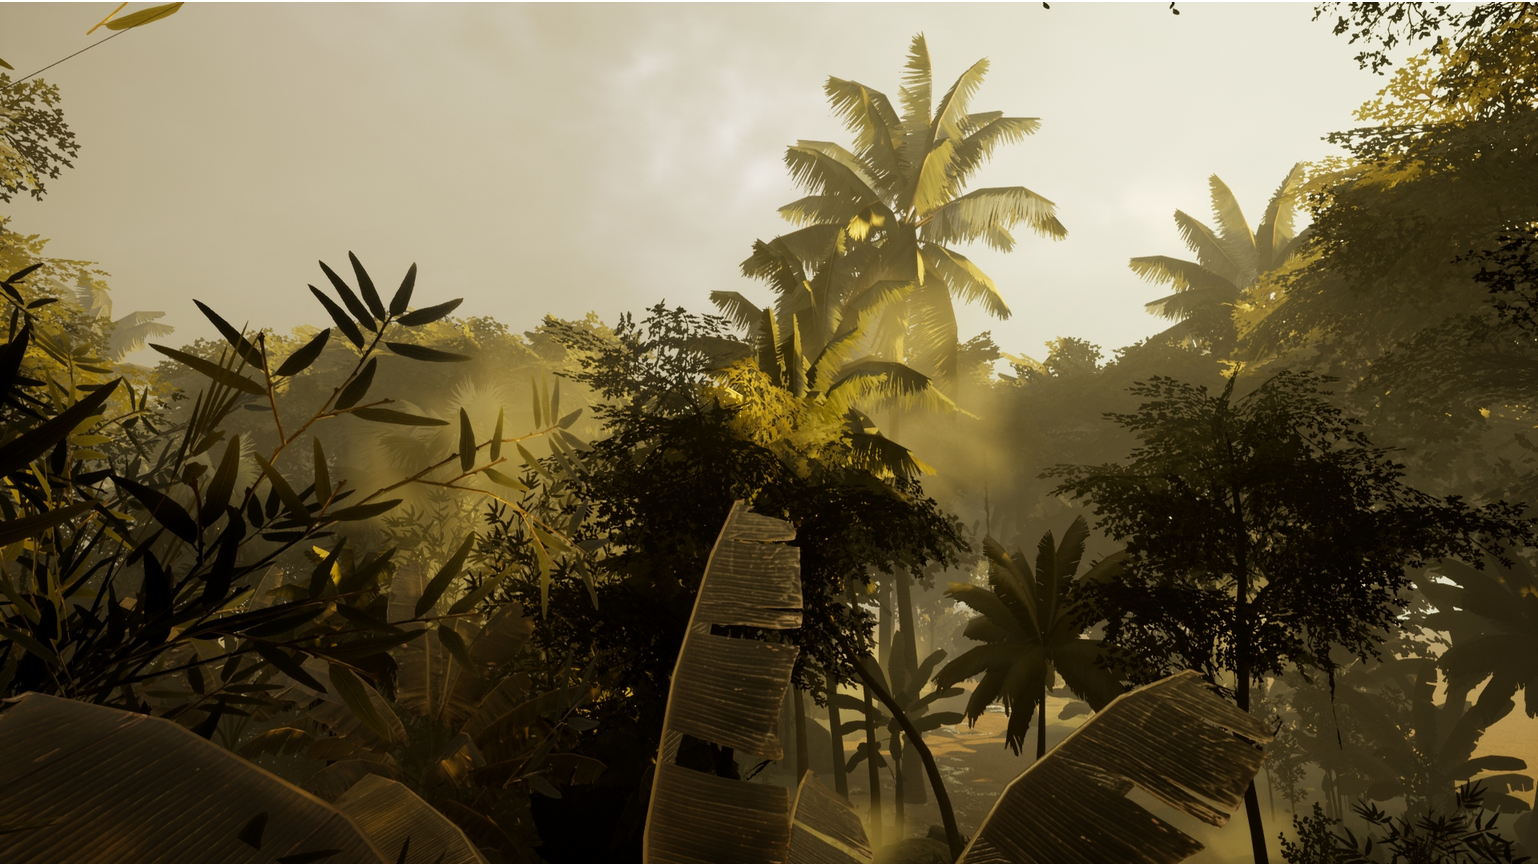
\includegraphics[width = 0.9\linewidth]{figs/UE4JungleProto.png}
%     \caption{Unreal Engine 4 Jungle Environment}
%     \label{fig:UE4JungleProto}
% \end{figure}
%\subsection{Security}



% \begin{figure}[h]
%     \centering
%     \includegraphics[width = 3 in]{figs/GazArena.png}
%     \caption{Gazebo Environment}
%     \label{fig:GazArena}
% \end{figure}

%andia National Labs considers examples where there is a compound that has a sensitive area that must be protected and is surrounded by land that contains wild life. Sometimes when an intruder is detected, the security system cannot determine if the threat is real or if there is simply an animal wandering around. A security officer must then go out and find the intruder to determine the state of the threat. In order to reduce wasted time, actively tracking that threat to provide the security personnel with a small region to search instead of a last known location saves resources. 

%and of security around a sensitive compound where tracking potential intruders is required for security personnel to make contact with and determine if the threat is real or false.




\subsection{Robot Platforms}

We use two robot simulation platforms to demonstrate the generality and applicability of the platform-agnostic methodology developed in this paper:
\begin{enumerate}
    \item An Iris quadcopter, which uses the PX4 flight stack and is capable of waypoint control.
    \item Stanley Innovations segway, which uses the ROS navigation stack for mapping, waypoint control, and autonomous obstacle avoidance. 
\end{enumerate}
To simulate the sensor output, we directly access the ground truth position of the moving target and add noise. We model the sensor and state estimation uncertainty as described in section \ref{sec:sensefunction} using a simulated 360 degree LiDAR with range of  $10$ meters, angular resolution of 1 degree, range accuracy of $\pm 3$ cm.


The function $vis$ is built directly from the sensor range parameter. To construct the function $sense$ we use a worst-case conservative Gaussian noise model. Given a sensor measurement, let $0 \leq p(l) \leq 1$ be the probability the target is in location $l$. We construct the uncertainty set $U$ of possible target states for each sensor measurement $sense(l_a,l_t)$ by including all states with a probability greater than $\delta$ where $0\leq \delta \leq 1$ can be set by the user. In the following simulations, we use $\delta = 0.95$. Informally, if a target is in sensor range, the agent's belief consists of \emph{all states} at which the target is with a probability greater than or equal to $5\%$. We note that, since the function $obs$ depends only on the sensors, the function needs to be constructed only once and can be used for all robots that use the same sensors. 
We test the synthesized surveillance strategies synthesized in two environments. One is an open urban-like setting modelled in Unreal Engine 4 depicted in Figure \ref{fig:UE4city}. A quadcopter acts as the surveilling agent and another acts as a potential intruder. In the second scenario, we consider an enclosed compound-like environment modelled in Gazebo as shown in Figure \ref{fig:GazArena}. The Iris quadcopter is tasked with tracking a hostile target (the Stanley Innovations segway) and maintaining sufficient knowledge of its location. We allow a human to directly control the rover and demonstrate the corresponding real-time response of the quadcopter to satisfy its surveillance task. We also perform the same experiment with the quadcopter controlled by a human and the Segway as the autonomous surveilling agent to emphasise that the framework is agnostic to the specific underlying hardware and can be easily applied. 
  
We contrast the surveillance needs and the qualitatively different resulting behaviours of the synthesized strategies for the agents in these two environments.

\begin{figure}
\centering


\subfloat[Urban environment modeled in Unreal Engine 4 \label{fig:UE4city}]{
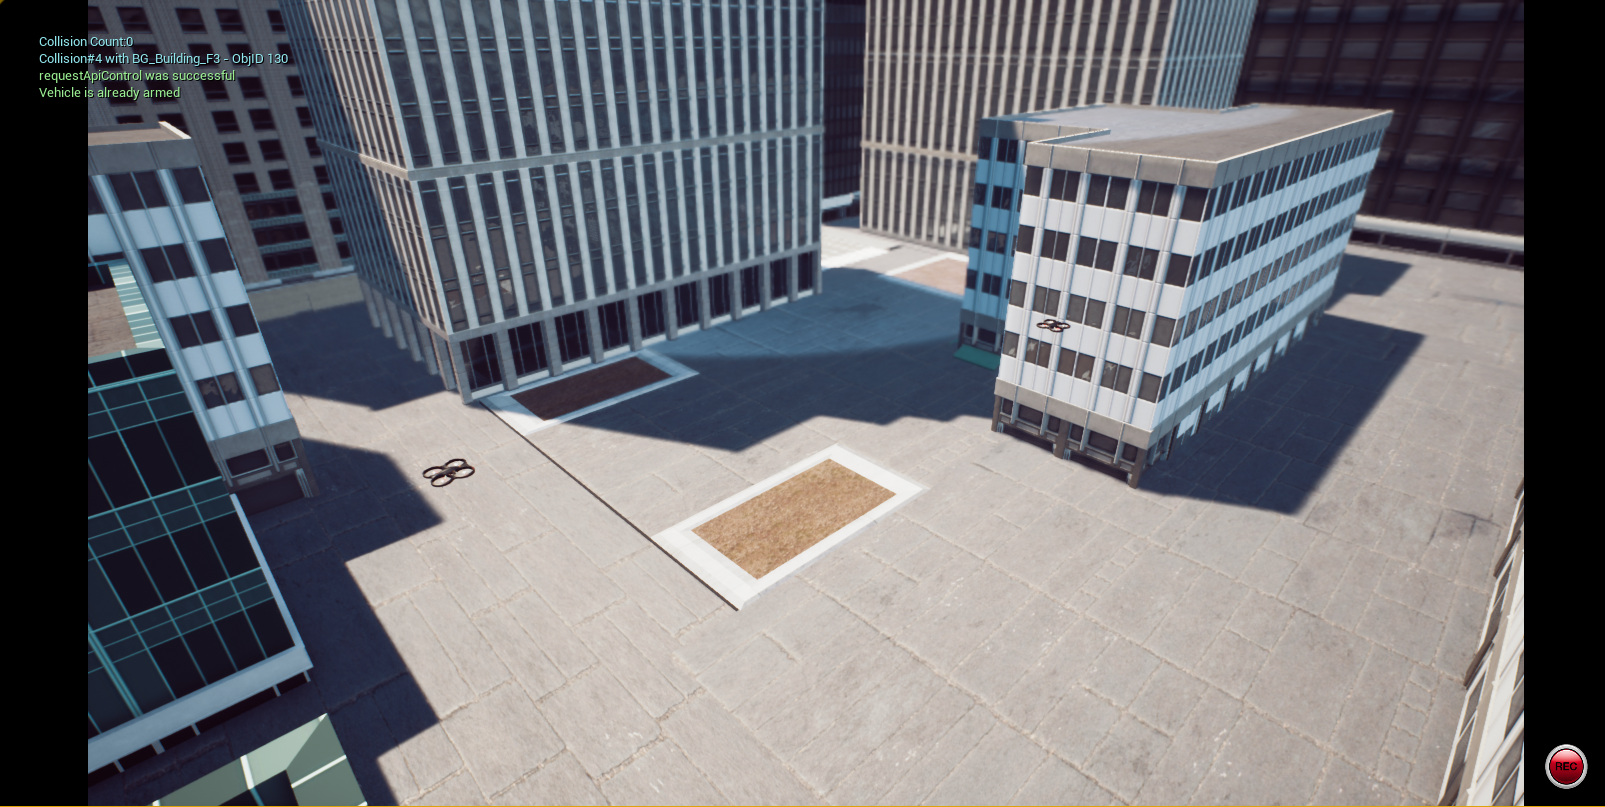
\includegraphics[width = 0.9\linewidth]{Surveillance/figs/unreal_city.png}}

\subfloat[Enclosed compound modelled in Gazebo \label{fig:GazArena}]{
\includegraphics[width = 0.9\linewidth]{Surveillance/figs/GazArena.png}}

\subfloat[Iris quadcopter used for autonomous surveillance \label{fig:sandiauav}]{
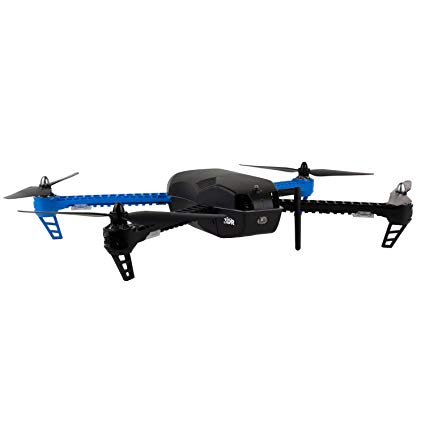
\includegraphics[width = 0.43\linewidth]{Surveillance/figs/quad.jpg}
} \hspace{0.05\linewidth}
\subfloat[Stanley innovations segway vehicle acting as a hostile target \label{fig:stanleyrobot}]{
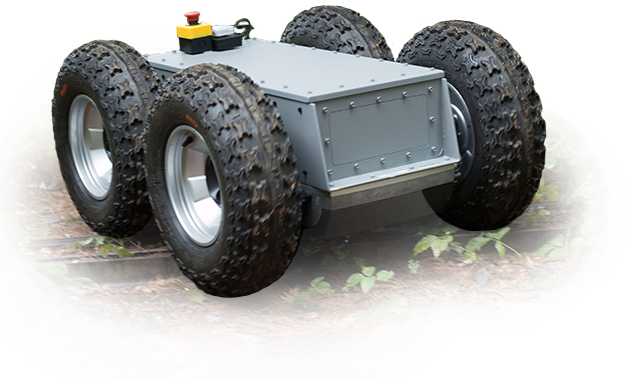
\includegraphics[width = 0.43\linewidth]{Surveillance/figs/Rugged-All-Terrain.png}
}

\caption{Case study for a security application. The vehicles are simulated in either Gazebo environment shown in \ref{fig:GazArena} or a UE4 environment shown in \ref{fig:GazArena}. A user can act as an `intruder' by controlling a target \ref{fig:stanleyrobot}. The UAV in \ref{fig:sandiauav} must autonomously react to guarantee the surveillance mission is satisfied. }
\label{fig:SandiaCaseSTudy}
\end{figure}